\section{\K 求解复杂电路的一般方法}

\subsection{\K 支路电流法}
\Par 根据网络拓扑学,如果一个完整电路有b条支路、n个节点、m个独立回路,那么它们有这样的关系
$$
b=m+n-1
$$
我们对n个节点可以列出n-1个节点KCL方程,对m个独立回路可以列出m个独立KVL方程,组成的基尔霍夫方程组可以解出b条支路电流.
\Par 对于每一回路根据KVL定律列出KVL方程,回路绕行方向与参考方向一致,KVL方程中该项的符号为正;绕行方向与参考方向相反,KVL方程中该项的符号为负.

\Par 对于每一节点根据KCL方程列出KCL方程,电流进入节点,KCL方程中该项的符号为正,电流离开节点,KCL方程中该项的符号为负.

\begin{wrapfigure}{r}{4.8cm}
    \centering
    \includegraphics[width=0.3\textwidth]{支路电流法.pdf}
    \caption{}
    \label{fig:支路电流法例题}
\end{wrapfigure}
\begin{example}\label{exp:支路电流法例题}
    如图\ref{fig:支路电流法例题}所示,$R_1=20\Omega ,R_2=5\Omega $,求电流$I_3$
\end{example}
\begin{solution}
如图\ref{fig:支路电流法例题}可以发现,有2个节点,2个网孔,因此我们可以列出含有3个独立方程的基尔霍夫方程组,其中包含2个KVL方程和1个KCL方程.
\begin{equation*}
    \begin{cases}
        I_1+I_2-I_3=0\\
        E_1-I_1R_1-I_3R_3=0\\
        I_3R_3+I_2R_2-E_2=0\\
    \end{cases}
\end{equation*}
代入相应的数值可以解得
\begin{equation*}
    \begin{cases}
        I_1=4A\\
        I_2=6A\\
        I_3=10A\\
    \end{cases}
\end{equation*}
\end{solution}

\subsection{\K 等效替换法}
\begin{table}[htbp]
    \centering
    \caption{电压源与电流源的比较}
    \begin{tblr}{row{odd} = {azure8,8.1em}, 
        row{even} = {gray8,8.1em},
        colspec={cccll},
        row{1} = {2em,azure2,fg=white},
        }
        名称 & 模型 & 特性方程 & 外特性曲线 & 理想条件\\
        电压源&\begin{minipage}[b]{0.18\columnwidth}
            \centering
            \raisebox{-.5\height}{\includegraphics[width=\linewidth]{电压源.pdf}}
        \end{minipage} &$U=E-IR_0$&\begin{minipage}[b]{0.18\columnwidth}
            \centering
            \raisebox{-.5\height}{\includegraphics[width=\linewidth]{电压源外特性曲线.pdf}}
        \end{minipage}&$R_0\to 0$\\
        电流源&\begin{minipage}[b]{0.18\columnwidth}
            \centering
            \raisebox{-.5\height}{\includegraphics[width=\linewidth]{电流源.pdf}}
        \end{minipage} &$U=\left( I_S-I \right) R_0$&\begin{minipage}[b]{0.18\columnwidth}
            \centering
            \raisebox{-.5\height}{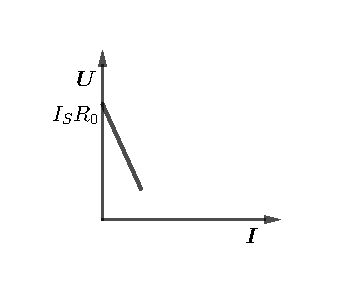
\includegraphics[width=\linewidth]{电流源外特性曲线.pdf}}
        \end{minipage}&$R_0\to \infty$\\
    \end{tblr}
\end{table}
\hl{电压源与电流源的等效替换:}从电压源与电流源两者的特性方程我们不难看出,当两方程的截距与斜率都相等的时候,即
\begin{equation*}
    \begin{array}{c}
        R_{V0}=R_{I0}\\
        E=I_SR_0\\
    \end{array}
\end{equation*}
两者可以等效替换.

回顾例题\ref{exp:支路电流法例题},我们这里用等效替换法再做一遍.

\begin{wrapfigure}{r}{4.8cm}
    \centering
    \includegraphics[width=0.3\textwidth]{等效替换法.pdf}
    \caption{}
    \label{fig:等效替换法}
\end{wrapfigure}
\begin{solution}
    我们将两个电压源等效替换为电流源,如图\ref{fig:等效替换法}所示,则有
    \begin{equation*}
        25A=I_1+I_2+I_3
    \end{equation*}
    其中,根据三个电阻的阻值关系(中间的是$R_3$)我们可以得到
    \begin{equation*}
        I_1:I_3:I_2=\frac{1}{R_1}:\frac{1}{R_3}:\frac{1}{R_2}=3:10:12
    \end{equation*}
    因此$I_3=10A$.
\end{solution}
\begin{remark}
    电流源适用于并联电路的求解,电压源适用于串联电路的求解.
\end{remark}

\subsection{\K 叠加原理}

\begin{theorem}[叠加原理]
    对于线性电路,任何一条支路中的电流,都可以看作是由电路中各个电源分别作用时,在此支路中所产生的电流的代数和.
\end{theorem}
\Par 重点解释一下定理中的几个名词:
\begin{enumerate}
    \item \hl{线性电路}:所谓线性电路,就是由线性元件组成的电路.而线性元件指的是满足欧姆定律的电子元件.非线性元件有:半导体二极管、真空二极管、气体导电管……而我们讨论的电阻就是典型的线性元件.
    \item \hl{代数和}:所谓代数和是指代数和式中每一项前面会有符号,符号表征了每一个分激励在该处利用叠加原理计算后得到的方向(注意,这里仍然是假定方向),同向则同号,反向则异号.具体的内容详见例题.
    \item \hl{注意事项}:叠加原理不能用来直接计算功率,因为功率的公式不是线性的.
\end{enumerate}

\begin{example}
    如图\ref{exp:支路电流法例题},$R_1=20\Omega ,R_2=5\Omega $,利用叠加原理求解$I_3$
\end{example}
\begin{solution}
    由于这两个电源都是电压源,因此我们对它们进行短接除源(见注释\ref{tips:除源})操作:

    先短接右边,以顺时针作为回路方向列出回路方程
    \begin{equation*}
        \left\{ \begin{aligned}
            &I_{1}^{'}=\frac{E_1}{R_1+\frac{R_2R_3}{R_2+R_3}}=\frac{140}{20+\frac{5\times 6}{5+6}}\mathrm{A}=6.16\mathrm{A}\\
            &I_{2}^{'}=\frac{R_3}{R_2+R_3}I_{1}^{'}=\frac{6}{5+6}\times 6.16\mathrm{A}=3.36\mathrm{A}\\
            &I_{3}^{'}=\frac{R_2}{R_2+R_3}I_{1}^{'}=\frac{5}{5+6}\times 6.16\mathrm{A}=2.80\mathrm{A}\\
        \end{aligned} \right. 
    \end{equation*}

    再短接左边,以逆时针作为回路方向列出回路方程
    \begin{equation*}
        \left\{ \begin{aligned}
            &I_{2}^{''}=\frac{E_2}{R_2+\frac{R_1R_3}{R_1+R_3}}=\frac{90}{5+\frac{20\times 6}{20+6}}\mathrm{A}=9.36\mathrm{A}\\
            &I_{1}^{''}=\frac{R_3}{R_1+R_3}I_{2}^{''}=\frac{6}{20+6}\times 9.36\mathrm{A}=2.16\mathrm{A}\\
            &I_{3}^{''}=\frac{R_1}{R_1+R_3}I_{2}^{''}=\frac{20}{20+6}\times 9.36\mathrm{A}=7.21\mathrm{A}\\
        \end{aligned} \right. 
    \end{equation*}
    \hl{注意},这里$I_{1}^{'},I_{2}^{'}$与$I_{1}^{"},I_{2}^{"}$的方向是相反的,因此这里作代数和时需注意\hl{符号}.
    \begin{equation*}
        \left\{ \begin{aligned}
            &I_1=I_{1}^{'}-I_{1}^{''}=(6.16-2.16)\mathrm{A}=4.0\mathrm{A}\\
            &I_2=I_{2}^{''}-I_{2}^{'}=(9.36-3.36)\mathrm{A}=6.0\mathrm{A}\\
            &I_3=I_{3}^{'}+I_{3}^{''}=(2.80+7.20)\mathrm{A}=10.0\mathrm{A}\\
        \end{aligned} \right. 
    \end{equation*}
\end{solution}

\begin{remark}
    这里的\hl{\hypertarget{除源}{除源}\label{tips:除源}}就是指排除电路中其他电源的干扰,单单分析一个电源的效果,具体的操作时,对电压源短接,电流源断开.
\end{remark}

\newpage
\subsection{\K 戴维宁定理}

\begin{definition}[二端网络]

    \begin{wrapfigure}{r}{6cm}
        \begin{center}
            \includegraphics[width=0.35\textwidth]{二端电路.pdf}
        \end{center}
        \caption{二端电路}
        \label{fig:二端电路}
    \end{wrapfigure}
    \Par 电路中任意划出来的、有两个引出端的部分称为一个\textbf{二端网络}.图\ref{fig:二端电路}中的N1和N2都是二端网络,由线性元件组成的网络称为\textbf{线性网络}.根据内部是否包含电源又可分为\textbf{无源二端网络}(如图\ref{fig:二端电路}中的N2)和\textbf{有源二端网络}(如图\ref{fig:二端电路}中的N1),网络两端之间的电压,称为\textbf{二端网络的电压};从一端流进(或流出)的电流,称为\textbf{二端网络的电流}.
    \end{definition}
    
    \Par 对于一个二端网络,无论它是有源的还是无源的,若将$N_1$替换成$N_1^{'}$,未替换部分的支路电流均没有改变,
    则称$N_1$与$N_1^{'}$\textbf{等效}.这是我们可以向一般情况推广,一个无源二端网络可以等效替换成一个电阻,
    这个电阻的阻值就是这个无源二端网络的\textbf{总阻值}或称\textbf{等效阻值};而一个有源二端网络可以替换成有适当电动势和内阻的电源.
    同时我们考虑极端情况下:
    \begin{enumerate}
        \item [\circledtext{1}] 一段理想无电阻导线可以等效替换为一个总阻值为0的无源二端网络;
        \item [\circledtext{2}] 一个断开的开关可以等效替换为一个总阻值为$+\infty$的无源二端网络.
    \end{enumerate}

\begin{theorem}[戴维宁定理]
\Par 等效电源的电动势$\boldsymbol{E}$就是有源二端网络的开路电压$U_0$,即,将负载断开后$a,b$两端之间的电压;等效电源的内阻$R_0$等于有源二端网络中所有电源均\hyperlink{除源}{除源}后所得到的无源网络$a,b$两端之间的等效电阻.
\end{theorem}

\begin{example}
    如图\ref{fig:等效前},$R_1=20\Omega ,R_2=5\Omega $,利用戴维宁定理求$I_3$.
\end{example}
\begin{solution}
    我们将$R_3$断开后得到两个节点$a,b$,为了得到等效电阻,我们对两个电阻做短接\hyperlink{除源}{除源}处理,可以发现$R_1,R_2$形成了并联,因此等效电阻为
    \begin{equation*}
        R_0=\frac{1}{\frac{1}{R_1}+\frac{1}{R_2}}=\frac{1}{\frac{1}{20}+\frac{1}{5}}=4\Omega 
    \end{equation*}
    将$R_3$断开后,两个电源和两个电阻构成了一个回路,我们对这个新电路分析可以发现,这个电路的电流为
    \begin{equation*}
        I=\frac{E_1-E_2}{R_1+R_2}=\frac{140-90}{20+5}=2\mathrm{A}
    \end{equation*}
    因此等效电压应该为
    \begin{equation*}
        U_0=IR_2+E_2=100\mathrm{V}
    \end{equation*}
    综上所述,可以得到$I_3$
    \begin{equation*}
        I_3=\frac{U_0}{R_0}=25\mathrm{A}
    \end{equation*}
    \hl{是吗?不对!我们还要将算出来的等效电压、电流代回到等效电路中!}

    如图\ref{fig:等效后},我们将等效电压、电流代回到等效电路中可以得到
    \begin{equation*}
        I_3=\frac{U_0}{R_0+R_3}=\frac{100}{4+6}=10\mathrm{A}
    \end{equation*}
    \begin{figure}[htbp]
        \centering
        \begin{minipage}{0.48\textwidth}
            \centering
            \includegraphics[height=0.18\textheight,width=0.8\textwidth]{支路电流法.pdf}
            \caption{等效前}
            \label{fig:等效前}
        \end{minipage}
        \begin{minipage}{0.48\textwidth}
            \centering
            \includegraphics[height=0.18\textheight,width=0.8\textwidth]{戴维宁定理等效后.pdf}
            \caption{等效后}
            \label{fig:等效后}
        \end{minipage}
    \end{figure}
\end{solution}
\begin{remark}
    一定要记得将算出来的等效电压、电流代回到等效电路中,然后计算出来的电流才是我们想要求的电流!
\end{remark}

